\documentclass[11pt, a4paper]{ISOM2700}
\usepackage{verbatim}
\usepackage{fancyhdr}
\usepackage{booktabs}
\usepackage{setspace}
\usepackage{amsmath,mathrsfs}
\usepackage{multicol}
\usepackage{amssymb}
\usepackage{graphicx}
\usepackage{caption}
\usepackage{subcaption}
\usepackage{array}
\usepackage{xcolor}
\usepackage{float}
\usepackage{enumitem}
\usepackage{mathcomp}
\usepackage{tabularx}
\usepackage{wasysym}
\usepackage{pbox}
\usepackage{tikz}
\usepackage{mathtools}
\usetikzlibrary{matrix}
\usepackage[normalem]{ulem}
\usepackage{multirow}
\usepackage[linesnumbered, ruled, boxed]{algorithm2e}
\SetKwRepeat{Do}{do}{while}

\title{Session 16}
\subtitle{Inventory Management III\\The Marriage of EOQ and Newsvendor}

\begin{document}
\begin{spacing}{1.5}
    
    \section{Overall introduction}

    {\bf EOQ Model}:
    \begin{itemize}
        \item Long lifecycle product(stable demand)
        \item tradeoff between {\it setup} and {\it holding costs}, driven by {\it frequency of ordering}
    \end{itemize}
    $$Q^\star = \sqrt{\frac{2DS}{H}},\ ROP=DL$$

    {\bf Newsvendor Model}
    \begin{itemize}
        \item Short lifecycle product(uncertain demand)
        \item tradeoff between {\it costs of excess leftover inventory} and {\it excess demand}.
    \end{itemize}
    $$\Pr(D\le Q^\star)=\frac{c_u}{c_u+c_o}\  {\rm (critical\ fractile)}$$

    In real world, nothing is certain. So how can we cooperate EOQ model with uncertain variables?

    \section{EOQ Model with Uncertain Demand}

    At Re-Order Point, we always use EOQ Model to decide how much to order. But in this way,
    uncertain demand may cause {\it overstocking} and {\it understocking}, in other words,
    ROP is no longer exactly a lead time before stock running out.

    How to determine ROP?
    \begin{itemize}
        \item $c_o$: cost of overstocking a unit, cost of holding one more unit
        \item $c_u$: cost of understocking a unit, ..
        \item Optimal ROP satisfies: $\disp \Pr(demand\ during\ lead\ time \le ROP)=\frac{c_u}{c_u+c_o}$
    \end{itemize}

    Normal Distribution, still, is a special case: 
    \begin{itemize}
        \item {\it Demand per unit time} is normally distributed with mean $D$ and SD $\sigma$
        \item Then, {\it demand during lead time} is normally distributed with mean $DL$ and SD $\sigma \sqrt{L}$
        (SD of demand for unit time is $\sigma$, so during lead time $L$: $\sqrt{\sigma^2+\sigma^2+\cdots +\sigma^2}=\sigma\sqrt{L}$)
        \item Then use Newsvendor Model, $ROP=DL+(\sigma\sqrt{L})\cdot z$, $DL$ is {\it ROP with deterministic demand},
        $\sigma\sqrt{L}$ is {\it safety stock}, if the demand is less failtile, safety stock is less.
    \end{itemize}

    [Example.] Demand is RV with mean 100 per week and SD 20. Orders arrive 0.5 week after ordering,
    fixed cost = 5000, holding cost = 4 per week. Suppose shop wants to maintain a service level of 85\%.

    (1) How much to order every time?

    $D=100,\sigma=20,L=0.5,S=5000,H=4, Q=\sqrt{\dfrac{2DS}{H}}=500$

    (2) When to reorder?

    $z=1.04$

    [Example.] Annual demand 15,600 units per year, weekly demand is 300 units with SD 90 units.
    Lead time is 4 weeks.

    (1) ROP to provide 98\% service level:

    $R=DL+\sigma\sqrt{L}\cdot z=1200+180*2.06=1570$ units.

    (2) If reduce safety stock by 50\%, the new service level? 

    $SS'=185$, $z=\dfrac{SS'}{\sigma\sqrt{L}}=1.03$,

    \section{EOQ Model with Quantity Discount}

    Goal: how can we cooperate EOQ model with quantity discount(when customer buys a lot)

    [Example.] Annual demand 40,000. Cost to process an order is 25, inv holding cost rate 
    is 20\%, given price schedule for product X.
    \begin{center}
        \begin{tabular}{c|c}
            \hline\hline
            \setstretch{0.5}
            {\bf Demand} & {\bf Unit Cost}\\\hline
            $\le 1500$ & 2.35\\\hline
            $1500<D\le 2500$ & 2.30\\\hline
            $2500<D\le 3000$ & 2.25\\\hline
            $D>3000$ & 2.20\\\hline\hline
        \end{tabular}
    \end{center}

    \begin{itemize}
        \item Start with lowest price, find the EOQ
        \item If the EOQ is not feasible, go to next higher level, solve the EOQ, $\cdots$
        \item Until you find EOQ falls in that interval
        \item Calculate total cost at EOQ and {\it every level breakpoint}, select the one with lowest cost.
    \end{itemize}

    At 2.20, EOQ=2,132 units, infeasible. At 2.25, EOQ=2,108 units, infeasible.
    At 2.30, EOQ=2,085 units, feasible.

    How to calculate {\bf total cost}?
    $$TC=DC+\frac{DS}{Q}+\dfrac{QH}{2}$$
    The last two terms are exactly the same in EOQ, $DC$: since now unit cost depends on quantity, 
    now we cannot ignore ordering cost anymore, because cost depends on how much you order. 
    Every cycle, $C\cdot Q$ costs, time interval is $Q/D$. $\frac{CQ}{Q/D}=CD$.

    For example, when 2085, $$TC=DC+\frac{DS}{Q}+\dfrac{QH}{2}=40000\cdot 2.30+\frac{40000\cdot 25}{2085}
    +\frac{2085\cdot (0.2\cdot 2.30)}{2}=92959$$

    In the example, $(2085, 92959), (2500, 90963), (3000, 88993)$, thus ordering 3000 is optimal.

    \section{Economic Production Quantity(EPQ) Model}

    In many cases, we cannot produce everything in one time slot. So how to incoorperate production?

    \begin{center}
        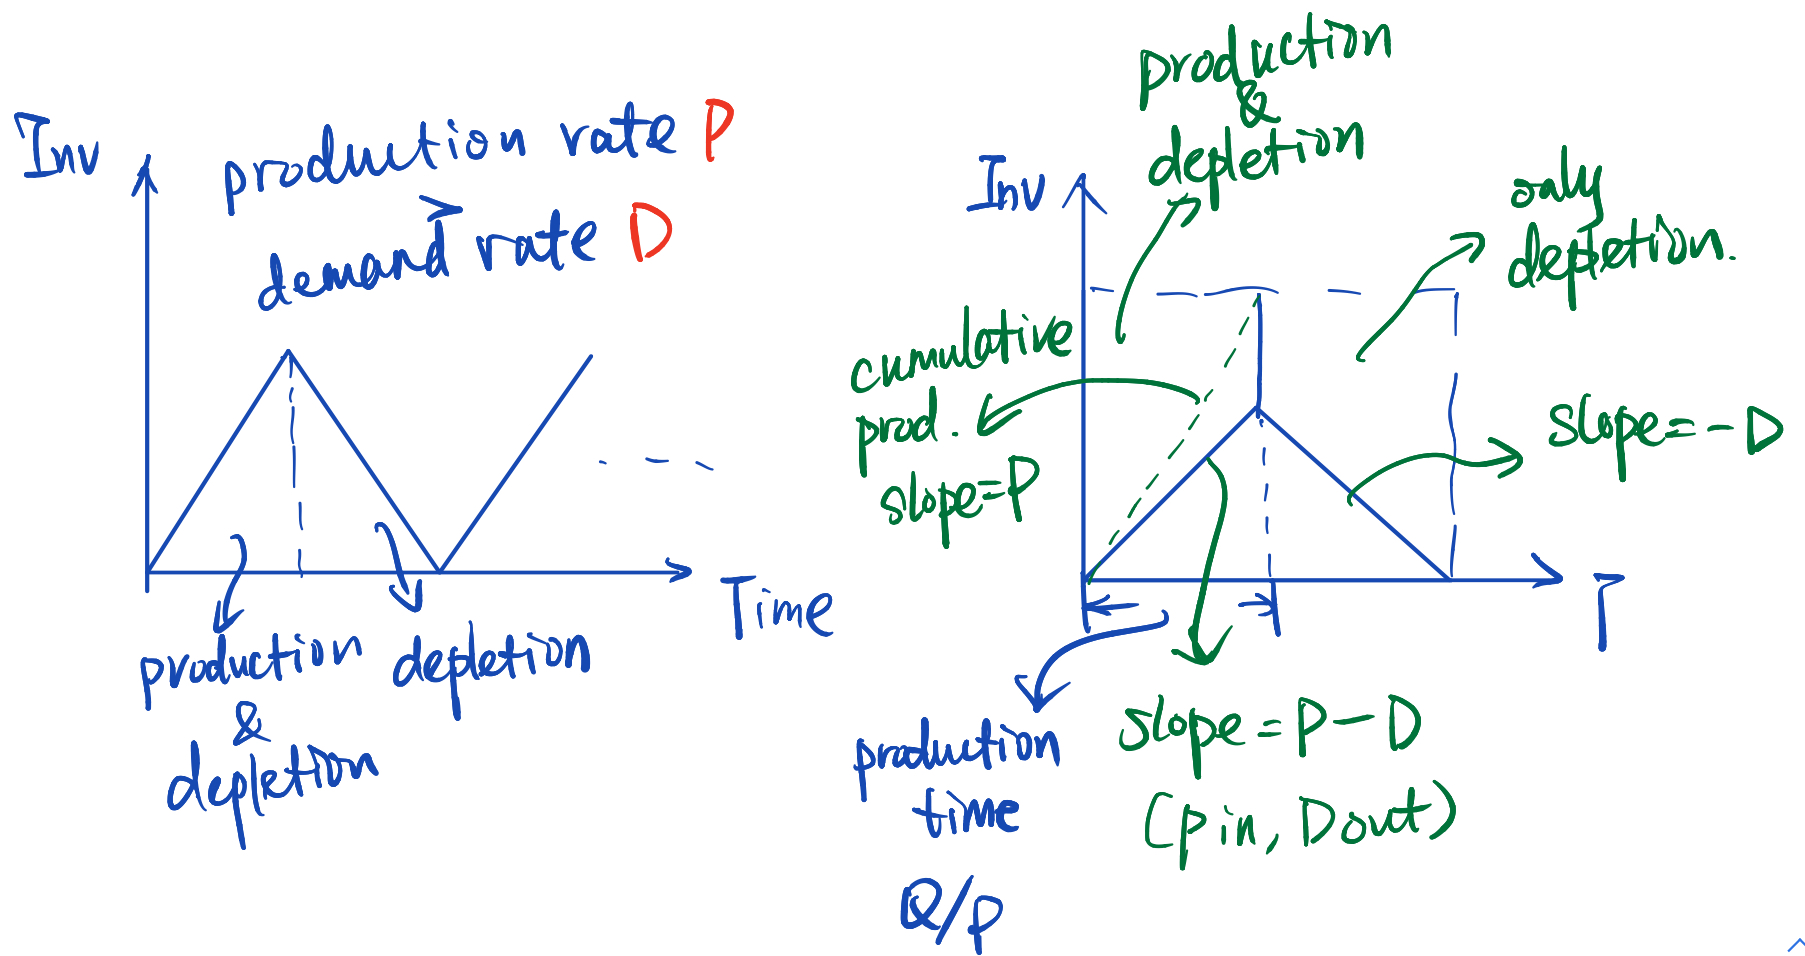
\includegraphics[scale=0.25]{images/S15-EPQ.jpeg}
    \end{center}

    Total Cost $\disp = TC(Q)=\frac{DS}{Q}+\frac{QH}{2}\left(1-\frac{D}{P}\right)$

    Find derivative, $Q^\star=\sqrt{\dfrac{2DS}{H\left(1-\frac{D}{P}\right)}}>\sqrt{\dfrac{2DS}{H}}$

    EOQ is actually a special case of this model. (when production rate tends to infinity)

    [Example.] Demand 1000 per week, produce rate 400 per week, 5000 fixed cost when start 
    production, margin cost 400, cost of capital 1\%.

    (1) $\disp Q^\star=\sqrt{\dfrac{2DS}{H\left(1-\frac{D}{P}\right)}}=
    \sqrt{\dfrac{2\cdot 100\cdot 5000}{4\cdot (1-1/4)}}=577$

    (2) Length of each production run: $\dfrac{Q^\star}{P}=1.44$ weeks.

    (3) Cycle time for optimal production quantity: $\dfrac{Q^\star}{D}=5.77$ weeks.

    \vspace{1in}
    {\it This is the end of lecture note. Last modified: Nov 2(during class).}

\end{spacing}
\end{document}
